\documentclass[conference]{IEEEtran}
\usepackage[T1]{fontenc}
\usepackage[utf8]{inputenc}
\usepackage[french]{babel}
\usepackage{cite}
\usepackage{amsmath,amssymb,amsfonts}
\usepackage{graphicx}
\usepackage{tikz}
\usetikzlibrary{arrows.meta,positioning}
\usepackage{booktabs}
\usepackage{array}
\usepackage{balance}
\usepackage[hidelinks]{hyperref}
\graphicspath{{figures/}{../results/}}
\renewcommand{\abstractname}{Résumé}
\renewcommand{\IEEEkeywordsname}{Mots-clés}
\renewcommand{\refname}{Références}
\newcommand{\minisection}[1]{\noindent\textbf{#1}}

\begin{document}

\title{Transmission d'images et de vidéos sur canal AWGN :\\
du codage classique au JSCC perceptuel}
\author{\IEEEauthorblockN{Eya Hammar, Yasmine Elhakem et Awab Zemzemi}}
\maketitle

\begin{abstract}
La transmission d'images sur un canal bruité impose un compromis entre
compression, robustesse et qualité de reconstruction. Le défi est de
préserver une image exploitable lorsque les perturbations du canal
altèrent sa représentation, tout en limitant les ressources de
transmission. Nous implémentons et étudions trois approches : une chaîne
numérique JPEG--Hamming--QPSK, un codage conjoint source--canal neuronal
optimisé par erreur quadratique moyenne et une seconde architecture
neuronale évaluée avec et sans perte perceptuelle fondée sur VGG16.
Toutes utilisent un canal gaussien blanc additif complexe. Une extension
vidéo traite 40 images à 10 FPS et évalue leur reconstruction ainsi
que la cohérence des prédictions d'un classificateur indépendant. Dans
l'expérience classique sauvegardée, Hamming permet de récupérer le JPEG
sans erreur à 10 et 12~dB, moyennant un surcoût de transmission de
75~\%. L'évaluation du JSCC sur une image atteint un PSNR de 21,27~dB
à un rapport signal sur bruit de 20~dB, contre 18,52~dB à 0~dB.
Dans l'étude distincte sur CIFAR-10, la variante perceptuelle atteint
27,68~dB de PSNR et 0,909 de SSIM à 20~dB, contre 26,30~dB et 0,870
pour sa référence MSE. Sur la séquence vidéo, les PSNR correspondants
sont de 21,64 et 21,27~dB à 20~dB ; les deux modèles atteignent
100~\% de cohérence sémantique à partir de 15~dB.
Ces résultats mettent en évidence des
comportements complémentaires, sans établir un classement global,
car les données et les budgets de transmission diffèrent. Nous
précisons les architectures, les protocoles et les limites nécessaires
à l'interprétation de ces mesures.
\end{abstract}

\begin{IEEEkeywords}
Transmission d'images, codage conjoint source--canal, DeepJSCC,
canal AWGN, correction d'erreurs, perte perceptuelle.
\end{IEEEkeywords}

\section{Introduction}
La communication visuelle sur une liaison bruitée impose de réduire
le volume transmis tout en maintenant une reconstruction exploitable.
Une chaîne classique sépare la compression de l'image et la protection
des bits. Des erreurs résiduelles dans un fichier JPEG peuvent
cependant entraîner des artefacts importants ou empêcher sa lecture.

Le codage conjoint source--canal neuronal (DeepJSCC) apprend directement
une représentation transmissible et sa reconstruction~\cite{deepjscc}.
Les pertes perceptuelles complètent l'erreur pixel par pixel par une
distance entre caractéristiques visuelles~\cite{perceptual}. Notre
problématique est d'étudier l'influence de ces choix sur la qualité
reçue et, pour une vidéo, sur la cohérence des prédictions sémantiques.

Nous implémentons une référence JPEG--Hamming--QPSK, un JSCC
convolutif orienté pixels et une architecture I/Q comparant MSE et
MSE avec perte perceptuelle. L'extension vidéo réutilise ces chaînes
image par image ; une séquence de 40 images est étudiée avec la
troisième approche. Les protocoles n'étant pas tous identiques,
nous distinguons les comparaisons internes d'un classement global.

La section~\ref{sec:related} présente l'état de l'art, la
section~\ref{sec:model} les architectures et fonctions de coût, puis
la section~\ref{sec:evaluation} les scénarios et résultats sur images
et vidéo. La section~\ref{sec:conclusion} conclut et expose les perspectives.

\section{État de l'art}
\label{sec:related}
\subsection{Compression et correction d'erreurs}
JPEG réduit les redondances des images, notamment par une compression
à pertes fondée sur la transformée en cosinus discrète~\cite{jpeg}.
Le codage de Hamming ajoute une redondance structurée pour corriger
certaines erreurs binaires~\cite{hamming}. Leur association constitue
une référence interprétable, mais sa protection reste limitée et
l'effet d'une erreur dépend de sa position dans le fichier. Notre
Hamming (7,4) est une base simple, non un code numérique optimisé.

\subsection{Codage conjoint neuronal}
Bourtsoulatze \textit{et al.} remplacent les codes explicites par deux
CNN séparés par une couche de canal non entraînable~\cite{deepjscc}.
Leur méthode transforme les pixels en symboles complexes et montre
une dégradation progressive avec le bruit. Notre JSCC syntaxique
reprend ce principe avec un objectif MSE et une architecture compacte ;
les performances publiées ne sont pas supposées acquises par cette
implémentation.

\subsection{Perception et information sémantique}
Johnson \textit{et al.} proposent des pertes fondées sur les
caractéristiques d'un réseau préentraîné~\cite{perceptual}. Nous
utilisons des couches gelées de VGG16~\cite{vgg}. Le SSIM évalue la
similarité structurelle et complète le PSNR~\cite{ssim}. Ces mesures
ne prouvent toutefois pas la conservation du sens d'une scène.
L'expérience vidéo les complète par la SPA, accord de prédiction
d'un CNN indépendant entre images originales et reconstruites.
Cet accord ne constitue pas une exactitude sur des annotations.

\section{Architecture et modèle proposé}
\label{sec:model}
\subsection{Vue d'ensemble des trois chaînes}
La figure~\ref{fig:architecture} présente les trois traitements
implémentés. La chaîne classique manipule un fichier JPEG et ses bits.
Les deux chaînes neuronales produisent directement des symboles et
reconstruisent une image. La troisième se distingue à la fois par son
architecture et par l'étude de la fonction de coût ; elle ne correspond
pas à l'ajout de VGG au même réseau que la deuxième approche.

\begin{figure*}[!t]
\centering
\begin{tikzpicture}[x=1cm,y=1cm,
block/.style={draw,rounded corners=2pt,align=center,font=\footnotesize,
minimum height=0.78cm,text width=2.05cm,fill=blue!5},
channel/.style={block,text width=1.45cm,fill=orange!13},
flow/.style={-{Latex[length=2mm]},thick}]
\node[anchor=west,font=\bfseries\small] at (-0.1,1.0)
{Approche 1 : traitement numérique séparé};
\node[block,text width=1.35cm] (a1) at (0.7,0) {Image RGB};
\node[block] (a2) at (3.0,0) {JPEG\\qualité 75};
\node[block] (a3) at (5.6,0) {Hamming (7,4)\\optionnel};
\node[block,text width=1.25cm] (a4) at (7.9,0) {QPSK};
\node[channel] (a5) at (10.1,0) {Canal AWGN};
\node[block,text width=3.0cm] (a6) at (13.2,0)
{Démodulation, décodage\\Hamming et JPEG};
\foreach \u/\v in {a1/a2,a2/a3,a3/a4,a4/a5,a5/a6}
\draw[flow] (\u) -- (\v);
\node[anchor=west,font=\bfseries\small] at (-0.1,-1.05)
{Approche 2 : JSCC orienté pixels, objectif MSE};
\node[block,text width=1.35cm] (b1) at (0.7,-2.05) {Image RGB};
\node[block] (b2) at (3.6,-2.05) {Encodeur CNN\\$16\times16\times16$};
\node[block,text width=2.3cm] (b3) at (6.8,-2.05)
{Normalisation\\2048 symboles complexes};
\node[channel] (b4) at (10.1,-2.05) {Canal AWGN};
\node[block,text width=3.0cm] (b5) at (13.2,-2.05)
{Décodeur CNN\\image reconstruite};
\foreach \u/\v in {b1/b2,b2/b3,b3/b4,b4/b5}
\draw[flow] (\u) -- (\v);
\node[anchor=west,font=\bfseries\small] at (-0.1,-3.1)
{Approche 3 : reconstruction neuronale, objectifs MSE ou MSE + perceptuel};
\node[block,text width=1.35cm] (c1) at (0.7,-4.1) {Image RGB};
\node[block] (c2) at (3.6,-4.1) {Encodeur CNN\\$2\times32\times32$};
\node[block,text width=2.3cm] (c3) at (6.8,-4.1)
{Normalisation I/Q\\1024 symboles complexes};
\node[channel] (c4) at (10.1,-4.1) {Canal AWGN};
\node[block,text width=3.0cm] (c5) at (13.2,-4.1)
{Décodeur CNN\\image reconstruite};
\foreach \u/\v in {c1/c2,c2/c3,c3/c4,c4/c5}
\draw[flow] (\u) -- (\v);
\end{tikzpicture}
\caption{Schéma des trois architectures. Les pertes comparent la
reconstruction à l'image d'entrée pendant l'entraînement. VGG16 sert
uniquement à calculer la perte perceptuelle ; il ne fait pas partie du
signal transmis ni du décodeur utilisé en inférence.}
\label{fig:architecture}
\end{figure*}

\subsection{Canal AWGN et contrainte de puissance}
Soit $x\in[0,1]^{3\times H\times W}$ une image RGB avec $H=W=128$.
L'encodeur neuronal produit $z=f_{\theta}(x)\in\mathbb C^K$.
La puissance est normalisée par image :
\begin{equation}
P_z=\frac1K\sum_{k=1}^{K}|z_k|^2,\qquad
\widetilde z_k=\frac{z_k}{\sqrt{P_z+\epsilon}},
\label{eq:power}
\end{equation}
où $\epsilon>0$ évite une division par zéro. Le canal fournit
\begin{equation}
y=\widetilde z+n,\qquad n_k\sim\mathcal{CN}(0,P/\gamma),
\label{eq:awgn}
\end{equation}
avec $P$ la puissance complexe moyenne et
$\gamma=10^{\mathrm{SNR}_{\mathrm{dB}}/10}$. Les composantes réelle
et imaginaire du bruit sont indépendantes, chacune de variance
$P/(2\gamma)$. Le décodeur produit $\widehat x=g_{\phi}(y)$.

La version complexe native du canal mesure la puissance d'entrée avant
de générer le bruit. La version à deux canaux réels I/Q normalise
d'abord la puissance, puis applique un bruit de puissance $1/\gamma$.
Les symboles QPSK ont une énergie unitaire. La simulation porte sur
la bande de base ; elle ne modélise pas une chaîne radio matérielle.

Nous explicitons le budget spatial par
\begin{equation}
\rho=\frac{K}{HW}.
\end{equation}
Il vaut $1/8$ pour le JSCC à 2048 symboles et $1/16$ pour
l'architecture à 1024 symboles. En comptant les trois composantes RGB
au dénominateur, ces rapports deviennent respectivement $1/24$ et
$1/48$. Ils ne représentent pas des rapports de taille de fichiers.

\subsection{Approche classique : JPEG, Hamming et QPSK}
L'image RGB redimensionnée est sauvegardée avant compression comme
référence. JPEG est appliqué avec une qualité de 75, puis les octets
sont convertis en bits. Pour chaque groupe de quatre bits utiles,
Hamming calcule
\begin{align}
p_1&=d_1\oplus d_2\oplus d_4,\\
p_2&=d_1\oplus d_3\oplus d_4,\\
p_4&=d_2\oplus d_3\oplus d_4.
\end{align}
Le mot transmis est $(p_1,p_2,d_1,p_4,d_2,d_3,d_4)$. Le récepteur
utilise le syndrome $s=s_1+2s_2+4s_4$ pour inverser la position
indiquée lorsqu'il est non nul. Cette correction suppose une erreur
unique par bloc ; plusieurs erreurs peuvent entraîner une mauvaise
correction.

La modulation QPSK emploie l'étiquetage de Gray
\begin{equation}
\begin{aligned}
00&\mapsto(1+j)/\sqrt2, & 01&\mapsto(-1+j)/\sqrt2,\\
11&\mapsto(-1-j)/\sqrt2, & 10&\mapsto(1-j)/\sqrt2.
\end{aligned}
\end{equation}
La démodulation choisit le point de constellation le plus proche.
Après éventuel décodage Hamming, les bits sont regroupés en octets
et le décodage JPEG est tenté intégralement. Un échec est conservé
comme résultat, sans lui attribuer de PSNR ou de SSIM artificiel.

Pour $L$ bits JPEG, la QPSK nécessite $L/2$ symboles sans FEC et,
hors remplissage, $7L/8$ avec Hamming, soit 75~\% de plus. Une
comparaison à SNR identique n'est donc pas une comparaison à budget
de transmission identique.

\subsection{JSCC convolutif orienté pixels}
L'encodeur comporte trois convolutions de noyau $5\times5$, de pas 2
et de remplissage 2, avec les canaux $3\to32\to64\to16$. Les deux
premières sont suivies de PReLU. Le tenseur latent
$16\times16\times16$ fournit 4096 valeurs réelles, regroupées par
paires en 2048 symboles complexes puis normalisées.

Le décodeur rétablit les composantes réelles et applique trois
convolutions transposées de noyau $4\times4$, de pas 2 et de
remplissage 1, avec les canaux $16\to64\to32\to3$. Deux PReLU et
une Sigmoid finale produisent une image dans $[0,1]$.

Les réseaux sont entraînés conjointement pour minimiser
\begin{equation}
\mathcal L_{\mathrm{MSE}}=
\frac1{3HW}\sum_{c,h,w}(x_{c,h,w}-\widehat x_{c,h,w})^2.
\label{eq:mse}
\end{equation}
Le canal est différentiable et un nouveau bruit est tiré à chaque
passage. Il ne possède aucun poids appris. Le SNR pilote le canal,
sans être fourni comme entrée supplémentaire aux réseaux.

\subsection{Architecture neuronale et extension perceptuelle}
La troisième architecture utilise trois convolutions $3\times3$,
les canaux $3\to32\to64\to2$ et les pas $2,2,1$. Deux ReLU
précèdent la sortie $2\times32\times32$, interprétée comme I et Q
pour 1024 symboles complexes. Le décodeur applique une convolution
$3\times3$ de 2 vers 64 canaux, puis deux convolutions transposées
$4\times4$ de pas 2, de 64 vers 32 puis 3 canaux. ReLU et Sigmoid
assurent respectivement la non-linéarité et la plage finale des pixels.

Deux modèles sauvegardés sont évalués : une référence MSE et une
variante dont l'objectif est
\begin{equation}
\mathcal L_{\mathrm{total}}=
\mathcal L_{\mathrm{MSE}}+\lambda\mathcal L_{\mathrm{perc}},
\qquad\lambda=0{,}01,
\end{equation}
où
\begin{equation}
\mathcal L_{\mathrm{perc}}=
\frac1M\left\|\psi(\mathcal N(x))-
\psi(\mathcal N(\widehat x))\right\|_1.
\end{equation}
$\mathcal N$ désigne la normalisation des canaux selon ImageNet,
$\psi$ les neuf premiers modules de caractéristiques de VGG16
préentraîné, et $M$ le nombre d'éléments comparés. Les poids VGG
sont gelés, mais le gradient sur l'image reconstruite est propagé
vers les réseaux de communication.

\section{Implémentation et évaluation des performances}
\label{sec:evaluation}
\subsection{Environnement de développement et données}
L'implémentation utilise Python, PyTorch pour les réseaux et le canal,
NumPy pour les bits, Pillow pour JPEG, scikit-image pour PSNR/SSIM et
Matplotlib pour les figures. Le JSCC orienté pixels est configuré
sur CPU. Le script perceptuel sélectionne CUDA si disponible, sinon
le CPU ; le matériel exact des expériences archivées n'est pas consigné.

L'expérience classique par défaut utilise \path{data/input.jpg}.
Une expérience complémentaire datée utilise
\path{data/test_images/test.png}, également employée pour les exemples
JSCC. Le JSCC charge les images locales de
\path{data/train_images/} et réalise une séparation aléatoire
entraînement/validation de 80/20 avec la graine 42. Le nombre exact
d'images ayant servi au modèle sauvegardé n'est pas établi par
l'historique seul.

L'étude perceptuelle charge les 5000 premières images d'entraînement
et les 1000 premières images de test de CIFAR-10~\cite{cifar}. Les
images natives $32\times32$ sont redimensionnées à $128\times128$ ;
cet agrandissement n'ajoute pas de détails originaux. Les étiquettes
de classe ne sont pas utilisées.

\subsection{Scénarios de test et paramètres}
Le tableau~\ref{tab:settings} rassemble les paramètres. Le meilleur
modèle JSCC est sélectionné selon la MSE de validation. Le script
perceptuel tire un SNR uniformément entre 0 et 20~dB pour chaque lot.
La comparaison MSE/perceptuel est disponible sous forme de résultats
archivés ; le script actuel n'établit pas à lui seul l'ensemble des
conditions d'entraînement de la référence MSE.

\begin{table*}[!t]
\centering
\caption{Paramètres d'implémentation et scénarios d'évaluation.}
\label{tab:settings}
\setlength{\tabcolsep}{5pt}
\begin{tabular}{p{3.4cm}p{3.6cm}p{3.8cm}p{4.5cm}}
\toprule
Paramètre & Approche classique & JSCC orienté pixels & Étude perceptuelle \\
\midrule
Résolution RGB & $128\times128$ & $128\times128$ & $128\times128$ après agrandissement \\
Données & Images locales & Images locales, séparation 80/20 & CIFAR-10 : 5000 / 1000 images \\
Compression ou latent & JPEG, qualité 75 & $16\times16\times16$ réel & $2\times32\times32$ réel \\
Symboles par image & Selon JPEG et FEC & 2048 complexes & 1024 complexes \\
Protection / objectif & Sans FEC ou Hamming (7,4) & MSE & MSE ou MSE + $0{,}01\mathcal L_{\mathrm{perc}}$ \\
Optimiseur / taux & Sans entraînement & Adam / 0,001 & Adam / 0,001\textsuperscript{a} \\
Taille du lot / époques & Sans entraînement & 4 / 10 & 32 / 3\textsuperscript{a} \\
SNR d'entraînement & Sans entraînement & 10 dB fixe & Uniforme $[0,20]$ dB\textsuperscript{a} \\
SNR de test (dB) & 5, 8, 10, 12 & 0, 5, 10, 15, 20 & $-5$, 0, 5, 10, 15, 20 \\
Répétitions du bruit & Une par configuration sauvegardée & Une, puis cinq par SNR et image & Un passage par SNR et modèle \\
\bottomrule
\end{tabular}
\par\smallskip\footnotesize
\textsuperscript{a}Paramètres du script actuel d'entraînement perceptuel.
L'entraînement complet du modèle MSE de référence n'est pas reconstitué.
\end{table*}

\subsection{Métriques et traçabilité des mesures}
Le BER mesure la fraction des bits JPEG utiles erronés, après
décodage Hamming lorsqu'il est activé. La lisibilité du fichier est
évaluée séparément. Pour des pixels normalisés, le PSNR vaut
\begin{equation}
\mathrm{PSNR}=10\log_{10}\left(\frac1{\mathrm{MSE}}\right).
\end{equation}
Sur des pixels entiers de 0 à 255, le numérateur devient $255^2$.
Le SSIM est calculé sur les images RGB~\cite{ssim}. Un PSNR et un
SSIM élevés sont préférables ; une perte perceptuelle faible est préférable.

L'inférence JSCC sur une image mesure les reconstructions après
arrondi en PNG 8 bits. L'évaluation répétée utilise directement les
pixels flottants. Pour chaque SNR, elle moyenne d'abord cinq bruits
par image, puis calcule la moyenne et l'écart-type entre images.
Le résumé sauvegardé ne contient qu'une image : les écarts-types
entre images sont donc fixés à zéro, sans démontrer une absence
de variation liée au bruit.

L'évaluation CIFAR-10 moyenne les PSNR et SSIM calculés par image.
La perte perceptuelle est pondérée par la taille des lots. Les deux
modèles utilisent les mêmes graines à chaque SNR, ce qui aligne les
bruits pour des lots et dimensions identiques.

Les résultats sur images proviennent des CSV sauvegardés du projet.
L'expérience vidéo de la section~\ref{sec:video} est décrite à partir
du protocole et des résultats communiqués par les auteurs.

\subsection{Résultats de l'approche classique}
Le tableau~\ref{tab:classical} présente l'expérience par défaut.
À 5~dB, Hamming réduit le BER de 0,03765 à 0,01202, mais aucun
JPEG n'est lisible. À 8~dB, les cinq erreurs restantes après FEC
suffisent encore à empêcher le décodage. À 10 et 12~dB, Hamming
récupère tous les bits du JPEG : le PSNR atteint 32,81~dB et le
SSIM 0,923. La différence avec l'image de référence provient alors
de la compression JPEG.

\begin{table}[!t]
\centering
\caption{Expérience classique par défaut. S : sans FEC ; H : Hamming.
Un tiret indique un JPEG illisible.}
\label{tab:classical}
\setlength{\tabcolsep}{3pt}
\begin{tabular}{rcrrrr}
\toprule
SNR & Mode & Erreurs & BER & PSNR & SSIM \\
(dB) & & & & (dB) & \\
\midrule
5 & S & 1084 & $3{,}765\!\times\!10^{-2}$ & --- & --- \\
5 & H & 346 & $1{,}202\!\times\!10^{-2}$ & --- & --- \\
8 & S & 169 & $5{,}870\!\times\!10^{-3}$ & --- & --- \\
8 & H & 5 & $1{,}737\!\times\!10^{-4}$ & --- & --- \\
10 & S & 34 & $1{,}181\!\times\!10^{-3}$ & --- & --- \\
10 & H & 0 & 0 & 32,81 & 0,923 \\
12 & S & 1 & $3{,}473\!\times\!10^{-5}$ & 15,40 & 0,826 \\
12 & H & 0 & 0 & 32,81 & 0,923 \\
\bottomrule
\end{tabular}
\end{table}

\begin{figure}[!t]
\centering
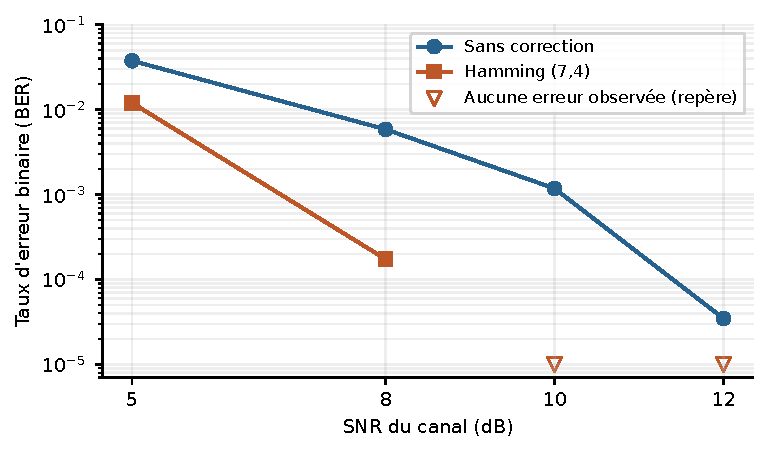
\includegraphics[width=\columnwidth]{classique_ber.pdf}
\caption{BER de l'expérience classique par défaut. Les triangles
signalent zéro erreur observée ; leur position à $10^{-5}$ est un
repère graphique et non une estimation du BER.}
\label{fig:ber}
\end{figure}

La figure~\ref{fig:ber} montre la baisse du BER avec le SNR et
l'amélioration apportée par Hamming dans cette expérience. Les zéros
observés à 10 et 12~dB ne garantissent pas un BER théorique nul.
À 12~dB sans FEC, une seule erreur laisse un JPEG lisible mais
dégradé, avec 15,40~dB de PSNR. Le nombre d'erreurs ne suffit donc
pas à décrire leur effet sur un fichier compressé.

La figure~\ref{fig:classical} provient d'une expérience complémentaire
sur l'image de test, conservée avec ses paramètres dans un dossier
daté. À 8~dB, Hamming laisse 13 erreurs, avec un JPEG décodable
mais un PSNR de seulement 10,90~dB. À 10~dB, il ne reste aucune
erreur et le PSNR atteint 31,98~dB, contre 10,36~dB sans FEC.
À 12~dB, les deux configurations récupèrent le fichier sans erreur.
Cette figure distingue visuellement un échec de lecture d'une
image lisible mais fortement altérée. Ses valeurs appartiennent à
un autre essai que celles du tableau~\ref{tab:classical}.

\begin{figure*}[!t]
\centering
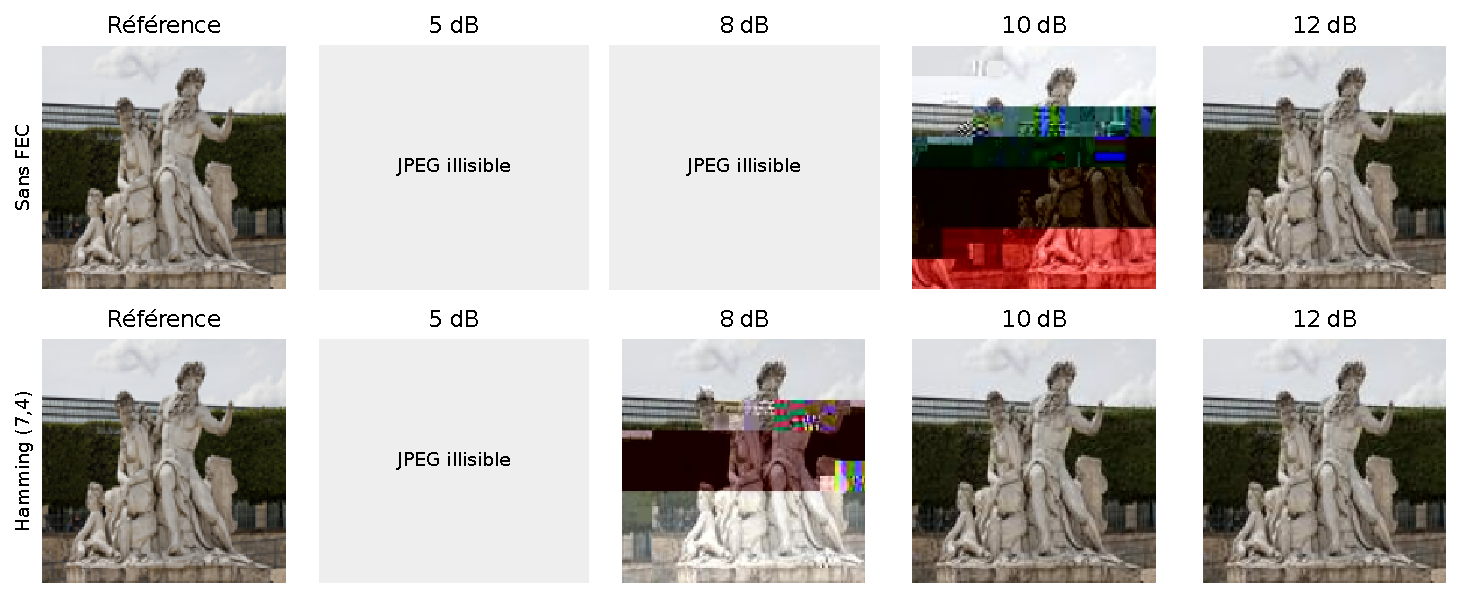
\includegraphics[width=0.85\textwidth]{classique_reconstructions.pdf}
\caption{Expérience classique complémentaire sur l'image de test :
référence et reconstructions avec et sans Hamming à 5, 8, 10 et
12~dB. Les cases grises indiquent les échecs de décodage JPEG.}
\label{fig:classical}
\end{figure*}

\subsection{Résultats du JSCC orienté pixels}
Le tableau~\ref{tab:jscc}
présentent l'évaluation sur une image. Entre 0 et 20~dB de SNR,
le PSNR passe de 18,52 à 21,27~dB et le SSIM de 0,453 à 0,608.
La moyenne des cinq transmissions suit la même tendance. Les
deux courbes ne constituent pas deux méthodes concurrentes : elles
utilisent le même modèle, mais des répétitions du bruit et une
représentation des pixels différentes pour le calcul des métriques.

\begin{table}[!t]
\centering
\caption{JSCC : une transmission et moyenne de cinq bruits sur une
image. Les métriques utilisent respectivement des pixels 8 bits et réels.}
\label{tab:jscc}
\setlength{\tabcolsep}{4pt}
\begin{tabular}{rrrrr}
\toprule
& \multicolumn{2}{c}{Une transmission} & \multicolumn{2}{c}{Moyenne répétée} \\
\cmidrule(lr){2-3}\cmidrule(lr){4-5}
SNR (dB) & PSNR (dB) & SSIM & PSNR (dB) & SSIM \\
\midrule
0 & 18,52 & 0,453 & 18,54 & 0,453 \\
5 & 20,31 & 0,539 & 20,24 & 0,537 \\
10 & 20,90 & 0,586 & 20,98 & 0,586 \\
15 & 21,21 & 0,602 & 21,19 & 0,601 \\
20 & 21,27 & 0,608 & 21,26 & 0,608 \\
\bottomrule
\end{tabular}
\end{table}



Le gain de PSNR entre 15 et 20~dB n'est que d'environ 0,06~dB
pour une transmission. Cette saturation est compatible avec une
limitation liée au modèle et à l'apprentissage, au-delà du bruit,
sans que les expériences permettent d'isoler ces causes.

La figure~\ref{fig:jsccimages} montre une reconstruction à chaque
SNR testé, y compris à 0~dB. La représentation continue évite
l'étape de lecture d'un fichier JPEG, mais les détails restent
imparfaits et les images floues. Produire une sortie ne garantit
donc pas la conservation de toutes les informations visuelles.

\begin{figure*}[!t]
\centering
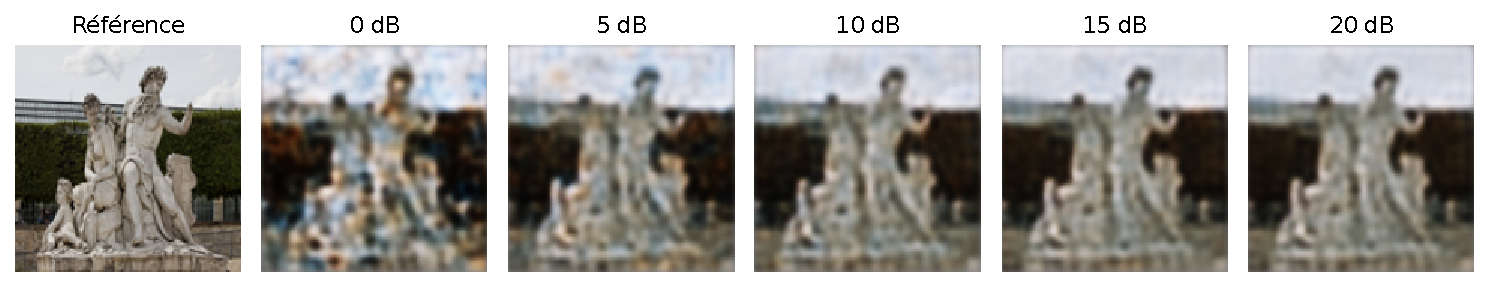
\includegraphics[width=0.97\textwidth]{jscc_reconstructions.pdf}
\caption{Référence et reconstructions du JSCC pour l'image de test.
Chaque transmission utilise 2048 symboles complexes et le même
modèle entraîné.}
\label{fig:jsccimages}
\end{figure*}

\subsection{Résultats de l'extension perceptuelle}
Le tableau~\ref{tab:perceptual} concerne les deux modèles de la
seconde architecture neuronale sur CIFAR-10. Le modèle perceptuel
présente un PSNR et un SSIM supérieurs, ainsi qu'une perte VGG
inférieure, à tous les SNR évalués. À 20~dB, le gain de PSNR
est de 1,37~dB et le SSIM augmente de 0,870 à 0,909.
La perte perceptuelle diminue d'environ 26,5~\%, de 0,513 à 0,377.

\begin{table*}[!t]
\centering
\caption{Résultats archivés sur CIFAR-10 : référence MSE et
extension perceptuelle de la même architecture I/Q. Une perte
perceptuelle plus faible est préférable.}
\label{tab:perceptual}
\begin{tabular}{r rrr rrr}
\toprule
& \multicolumn{3}{c}{Référence MSE}
& \multicolumn{3}{c}{MSE + $0{,}01\mathcal L_{\mathrm{perc}}$} \\
\cmidrule(lr){2-4}\cmidrule(lr){5-7}
SNR (dB) & PSNR (dB) & SSIM & Perte perceptuelle
& PSNR (dB) & SSIM & Perte perceptuelle \\
\midrule
$-5$ & 16,39 & 0,362 & 1,211 & 16,43 & 0,395 & 1,069 \\
0 & 20,23 & 0,559 & 0,931 & 20,40 & 0,600 & 0,804 \\
5 & 23,33 & 0,721 & 0,730 & 23,78 & 0,763 & 0,606 \\
10 & 25,17 & 0,814 & 0,606 & 26,03 & 0,855 & 0,479 \\
15 & 26,00 & 0,855 & 0,541 & 27,20 & 0,894 & 0,409 \\
20 & 26,30 & 0,870 & 0,513 & 27,68 & 0,909 & 0,377 \\
\bottomrule
\end{tabular}
\end{table*}

\begin{figure*}[!t]
\centering
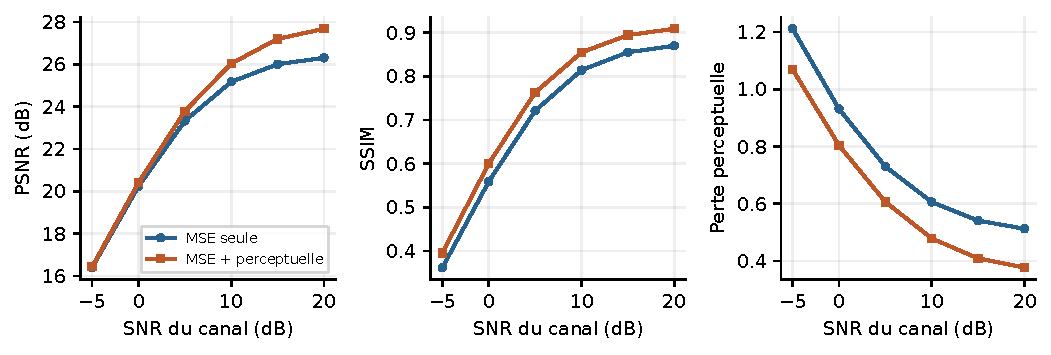
\includegraphics[width=0.90\textwidth]{perceptuel_qualite.pdf}
\caption{Comparaison de la référence MSE et de l'extension
perceptuelle sur CIFAR-10 : PSNR, SSIM et perte perceptuelle.
Ces courbes décrivent les modèles sauvegardés, sans moyenne sur
plusieurs entraînements indépendants.}
\label{fig:perceptual}
\end{figure*}

La figure~\ref{fig:perceptual} rend visible l'amélioration des
trois indicateurs. À $-5$~dB, le gain de PSNR est toutefois
limité à environ 0,04~dB, alors que le SSIM et la distance VGG
s'améliorent davantage. Les avantages observés dépendent donc
du niveau de bruit et du critère considéré.

La distance VGG utilisée pour évaluer est aussi présente dans
l'objectif d'entraînement. Sa baisse est cohérente avec cet
objectif, mais ne constitue pas une validation indépendante de la
perception humaine ou de la préservation sémantique. De plus,
l'absence de plusieurs entraînements et de la provenance complète
du modèle MSE limite l'attribution causale des écarts à la seule perte.

\subsubsection{Comparaison des images reconstruites}
La figure~\ref{fig:perceptualreconstructions} présente les sorties
visuelles de la troisième approche. Elle montre, pour une même
image CIFAR-10, la référence,
la reconstruction du modèle MSE et celle du modèle MSE avec perte
perceptuelle, à $-5$, 0, 10 et 20~dB. Les lignes suivent cet ordre de
SNR de haut en bas. Cette figure est issue du résultat sauvegardé
\path{results/reconstruction_comparison_001.png}, sans nouvelle inférence.

Aux deux SNR les plus faibles, les deux reconstructions présentent
des déformations importantes. Lorsque le SNR augmente, la silhouette
et les grandes régions de couleur deviennent plus proches de la
référence. Des différences entre les deux modèles restent visibles,
mais cet exemple seul ne permet pas de quantifier un gain général.
Il complète les moyennes du tableau~\ref{tab:perceptual} et les
courbes de la figure~\ref{fig:perceptual}, qui portent sur le
sous-ensemble de test. Les deux colonnes reconstruites utilisent les
mêmes graines de bruit pour chaque SNR, conformément au script
de visualisation.

\begin{figure}[!t]
\centering
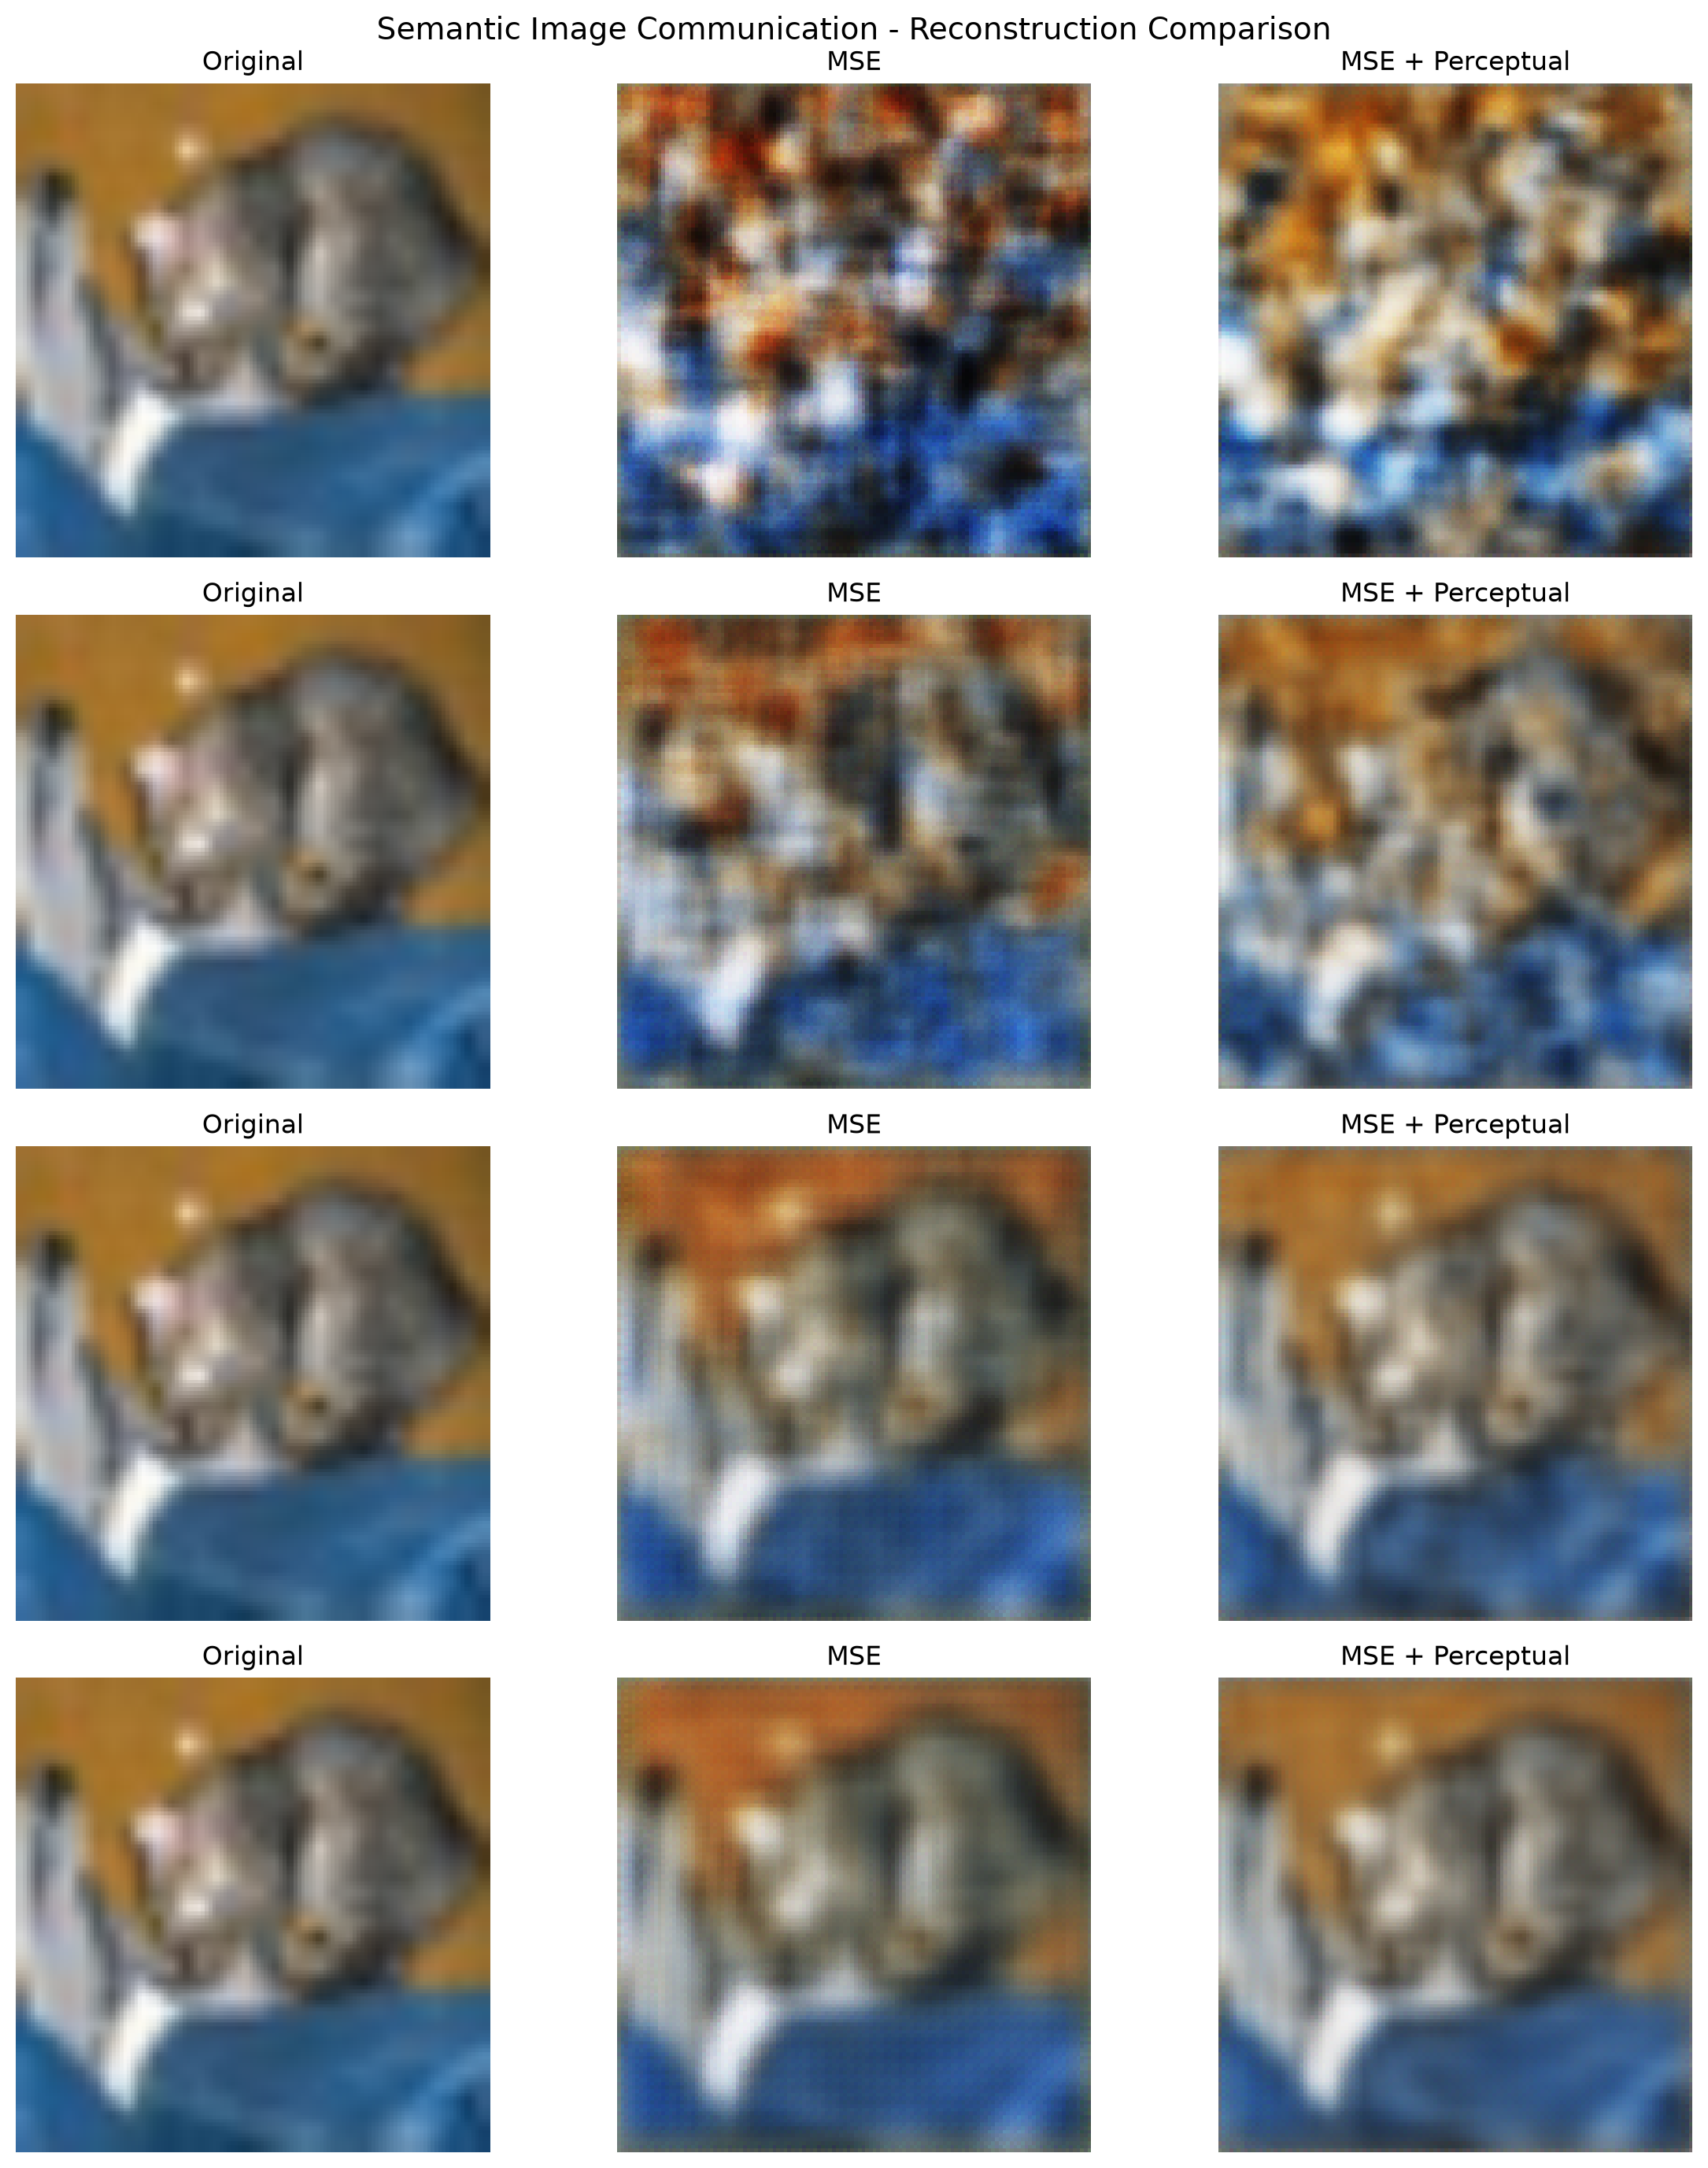
\includegraphics[width=0.88\columnwidth]{reconstruction_comparison_001.png}
\caption{Sorties visuelles de la troisième approche sur une image
CIFAR-10. Colonnes de gauche à droite : image de référence, modèle
MSE seul et modèle MSE avec perte perceptuelle. Lignes de haut en
bas : SNR de $-5$, 0, 10 et 20~dB. Les intitulés anglais sont ceux
de la figure originale sauvegardée.}
\label{fig:perceptualreconstructions}
\end{figure}

\subsection{Extension à la communication vidéo}
\label{sec:video}
\subsubsection{Protocole expérimental}
Le système d'images est étendu à une vidéo MP4 dont 40 images sont
extraites avec OpenCV à une cadence de 10 FPS. Chaque image est
convertie en RGB, redimensionnée à $128\times128$, puis transmise
indépendamment par le même encodeur, canal AWGN et décodeur que
pour les images. La séquence traitée représente quatre secondes.
Les paramètres sont résumés dans le tableau~\ref{tab:video}.

Le sélecteur logiciel permet les trois approches. L'expérience vidéo
rapportée ici porte spécifiquement sur la troisième : les variantes
MSE seule et MSE avec perte perceptuelle de l'architecture I/Q.
Les réseaux sont utilisés en évaluation, sans nouvel entraînement.
Une vidéo est reconstruite à 10 FPS pour chaque SNR ; les images
restent indépendantes, sans prédiction inter-image ni estimation de
mouvement. Les sorties de présentation utilisent Motion-JPEG AVI.

\begin{table}[!t]
\centering
\caption{Protocole de l'expérience vidéo de la troisième approche.}
\label{tab:video}
\begin{tabular}{ll}
\toprule
Paramètre & Configuration \\
\midrule
Entrée / cadence & MP4, 40 images, 10 FPS \\
Résolution & RGB $128\times128$ \\
Variantes & MSE ; MSE + perte perceptuelle \\
SNR (dB) & $-5$, 0, 5, 10, 15, 20 \\
Mesures & PSNR, SSIM, SPA \\
Transmission & Images indépendantes \\
\bottomrule
\end{tabular}
\end{table}

\subsubsection{Qualité visuelle et préservation sémantique}
PSNR et SSIM sont mesurés par image puis moyennés sur les
40 images. La \emph{Semantic Preservation Accuracy} (SPA) mesure
l'accord entre les prédictions d'un classificateur CNN indépendant
sur l'image originale et sur sa reconstruction :
\begin{equation}
\mathrm{SPA}_s=\frac{100}{T}\sum_{t=0}^{T-1}
\mathbf{1}\!\left[C(x_t)=C(\widehat{x}_{t,s})\right],\quad T=40.
\end{equation}
$C$ désigne le classificateur fixé et $\mathbf{1}$ l'indicatrice.
La SPA mesure une cohérence de décision ; un accord peut aussi
survenir lorsque les deux prédictions sont incorrectes. Elle ne
remplace donc pas une exactitude calculée sur des annotations.

Selon les résultats communiqués pour cette expérience, la qualité
augmente avec le SNR et la variante perceptuelle obtient les
meilleures mesures de reconstruction sur les six valeurs testées.
Le tableau~\ref{tab:videoresults} présente les scores disponibles
à 20~dB : le PSNR passe de 21,27 à 21,64~dB, soit un gain de
0,37~dB, et le SSIM de 0,750 à 0,785, soit un gain de 0,035.
Les deux variantes atteignent une SPA de 100~\% à partir de 15~dB.
Cette égalité en SPA coexiste donc avec des différences de fidélité
visuelle. Les valeurs détaillées aux autres SNR ne sont pas extrapolées.

\begin{table}[!t]
\centering
\caption{Résultats vidéo à 20~dB, communiqués par les auteurs.
PSNR et SSIM moyens sur 40 images.}
\label{tab:videoresults}
\setlength{\tabcolsep}{5pt}
\begin{tabular}{lrrr}
\toprule
Modèle & PSNR (dB) & SSIM & SPA (\%) \\
\midrule
MSE & 21,27 & 0,750 & 100 \\
MSE + perceptuelle & 21,64 & 0,785 & 100 \\
\bottomrule
\end{tabular}
\end{table}

Ces observations étendent l'étude d'images à une courte séquence
vidéo et suggèrent l'intérêt de l'objectif perceptuel pour la
reconstruction. Elles restent limitées à 40 images corrélées d'une
même vidéo et au classificateur utilisé. La redondance temporelle
n'est pas exploitée par la transmission.

\subsection{Discussion comparative}
Les expériences classiques mettent en évidence la sensibilité des
fichiers compressés aux erreurs résiduelles et le bénéfice d'une
protection redondante. Le JSCC produit directement une image à
partir des symboles reçus, avec une qualité qui évolue avec le bruit.
La comparaison perceptuelle montre une amélioration des mesures
de reconstruction pour les deux modèles CIFAR-10 disponibles.

Ces observations ne justifient pas un classement global : les jeux
de données, les architectures, les SNR d'entraînement et les budgets
de symboles diffèrent. En particulier, le JSCC emploie 2048 symboles
par image, l'étude perceptuelle 1024, et la chaîne classique une
quantité dépendant du JPEG et du FEC. Même les exemples portant
sur une image commune ne sont pas comparés à budget égal.

\section{Conclusion et perspectives}
\label{sec:conclusion}
Nous avons implémenté trois chaînes de transmission d'images sur
canal AWGN et analysé leurs résultats sauvegardés. La chaîne
classique rend explicites les rôles de JPEG, Hamming et QPSK.
Hamming permet une récupération sans erreur à 10 et 12~dB dans
l'expérience par défaut, avec un surcoût de 75~\%. Le JSCC
convolutif atteint 21,27~dB de PSNR à 20~dB sur l'image évaluée.
Dans l'étude CIFAR-10 distincte, le modèle perceptuel atteint
27,68~dB et un SSIM de 0,909, contre 26,30~dB et 0,870 pour
sa référence MSE.

Sur la vidéo de 40 images à 10 FPS, la variante perceptuelle atteint
21,64~dB de PSNR et 0,785 de SSIM à 20~dB. Les deux modèles
conservent les prédictions du classificateur pour toutes les images
à partir de 15~dB ; cette observation reste propre à la séquence évaluée.

Les principales limites sont l'hétérogénéité des protocoles, une
seule image dans l'évaluation JSCC répétée et l'absence de plusieurs
graines d'entraînement. La documentation complète des conditions
d'entraînement reste nécessaire à l'interprétation des comparaisons.

La prochaine étape consiste à imposer les mêmes images de test,
la même puissance et le même nombre de symboles aux trois
approches. Elle devra intégrer des codes correcteurs plus puissants,
plusieurs entraînements et des intervalles d'incertitude. Des canaux
avec évanouissement et des contraintes matérielles rapprocheraient
la simulation d'une liaison réelle. Enfin, l'évaluation devrait étendre la SPA à plusieurs vidéos et
classificateurs, inclure des annotations de référence et étudier
l'exploitation de la redondance temporelle entre images.

\bibliographystyle{IEEEtran}
\bibliography{paper-references}

\end{document}
